\documentclass{article}
\usepackage[left=2cm,right=2cm,top=2cm,bottom=2cm]{geometry}
\usepackage[utf8]{inputenc}
\usepackage[german]{babel}
\usepackage{amsmath}
\usepackage{dsfont}
\usepackage[export]{adjustbox}
\usepackage{amsthm}
\usepackage{color}
\usepackage{amsfonts}
\usepackage{amssymb}
\usepackage{wasysym}
\usepackage{makeidx}
\usepackage{graphicx}
\usepackage[colorlinks=true,urlcolor=blue,linkcolor=blue]{hyperref}
\usepackage{ziffer}
\usepackage{minted}
\usepackage{xcolor}
\usepackage{framed}
\usepackage{mdframed}
\usepackage{subfiles}
\usemintedstyle{emacs}

\definecolor{purp}{HTML}{9A72AC}
\definecolor{re}{HTML}{FC6255}
\definecolor{gre}{HTML}{83C167}
\definecolor{blu}{HTML}{58C4DD}
\definecolor{shadecolor}{rgb}{0.85,0.85,0.85}
\definecolor{bg}{rgb}{0.95,0.95,0.95}
\setlength{\parindent}{0em} 

\BeforeBeginEnvironment{minted}{\begin{mdframed}[linewidth =2 ,backgroundcolor=bg , linecolor=black, linewidth=0.5]}
\AfterEndEnvironment{minted}{\end{mdframed}}

\newtheorem{defi}{Definition}
\BeforeBeginEnvironment{defi}{\begin{mdframed}[linewidth =2 ,backgroundcolor=bg , linecolor=black, linewidth=0.5]}
\AfterEndEnvironment{defi}{\end{mdframed}}

\newcommand{\bsp}{\textbf{Beispiel}:}
%\newcommand{\task}{\textbf{Aufgabe}:}

\newcommand{\bol}[1]{\textbf{#1}}
\newcommand{\q}[1]{\glqq #1\grqq}
\newcommand{\DODO}[1]{\textbf{\textcolor{red}{DODO:}} #1 \\ \begin{center}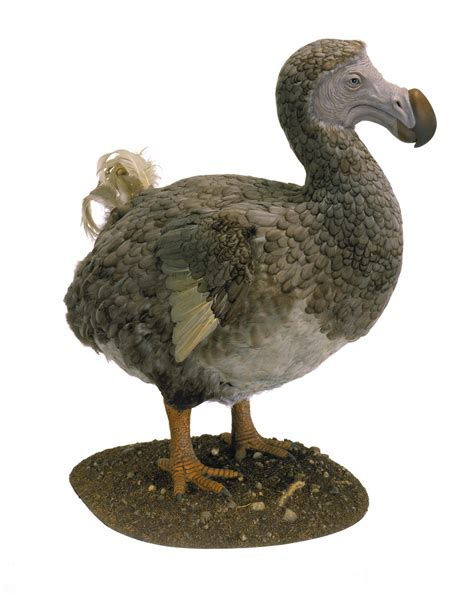
\includegraphics[scale=0.2]{../../media/dodo.jpg} \end{center}}

\newenvironment{task}[1]{
    \begin{shaded*}
    \textbf{Aufgabe #1}:
}{
    \end{shaded*}
}

\begin{document}

\subsection{Klassendiagramme}

Ein Klassendiagramm enthält eine Klassenkarte für alle beteiligten Klassen, sowie Pfeile zwischen ihnen, um die Beziehungen zu veranschaulichen. Für das Abitur wird noch zwischen erweiterten Klassendiagrammen und \q{normalen} Klassendiagrammen unterschieden. Das reguläre Diagramm enthält:
\begin{itemize}
    \item Attribute (nur Bezeichner)
    \item Methoden mit den Übergabeparametern (Bezeichner)
    \item Beziehungen zwischen Klassen, Referenzen werden auf Verbindungen modelliert, inklusive Mengenangaben.
    \item i.d.R. ohne Geben- und Setzen- Methoden
\end{itemize}
Für das erweiterte Klassendiagramm zusätzlich:
\begin{itemize}
    \item Datentypen der Attribute
    \item ggf. Referenzattribute 
    \item Rückgabewerte der Parameter 
    \item Konstrukturen
\end{itemize}
Vererbungen werden als Pfeile mit nicht-ausgemalter Spitze dargestellt. Abstrakte Klassen und Interfaces werden kursiv dargstellt oder (einfacher zu zeichnen) mit $<<$abstract$>>$ bzw. $<<$interface$>>$ gekennzeichnet. Werden Interfaces implementiert, so sieht der Pfeil aus wie bei einer Vererbung, allerdings gestrichelt. \\
Folgendes Beispiel aus dem Skript enthält die meisten relevanten Elemente als Beispiel.
\begin{center}
    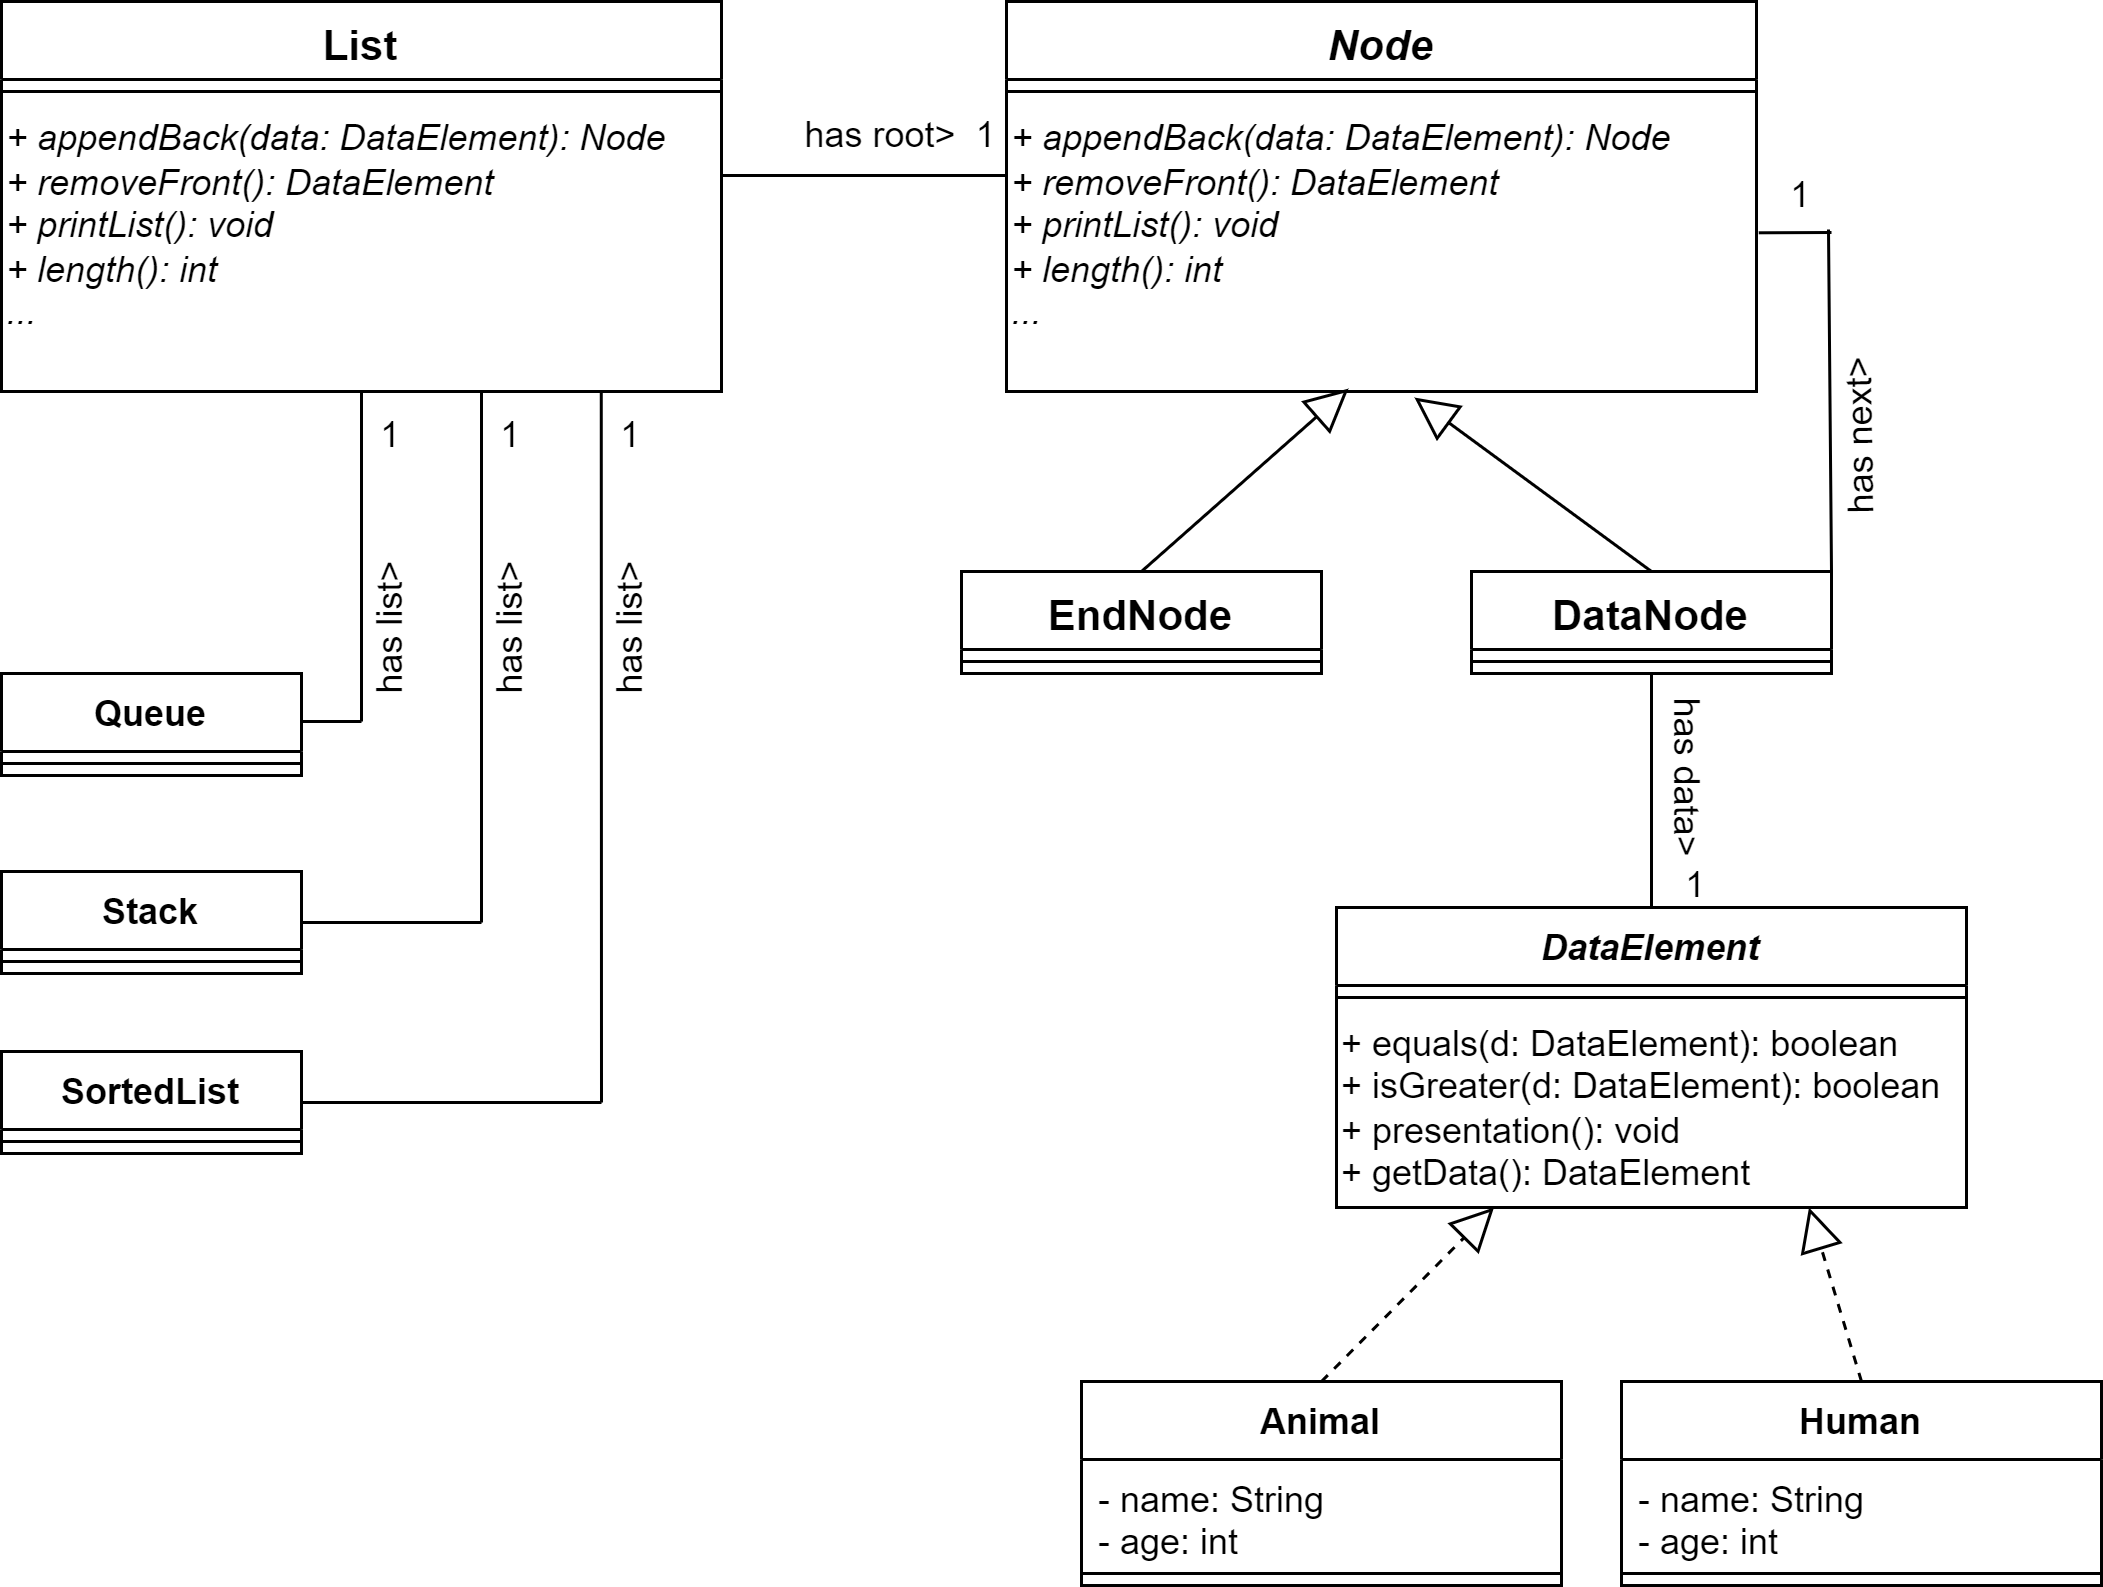
\includegraphics[scale=0.2]{../media/adapter_lists.png}
\end{center}
\textit{Hinweis:} Im Zweifelsfall schadet mehr Information im Diagramm nicht. Das erweiterte Klassendiagramm ist zu bevorzugen. 
\subsection{Objektdiagramme}

Im Gegensatz zum Klassendiagramm, das die allgemeine Struktur der Implementierung darstlelen soll, stellt das Objektdiagramm den Zustand des Systems zu einem bestimmtem Zeitpunkt dar.  \\ 
Das folgende Beispiel zeigt den Zustand einer Liste zu einem bestimmten Zeitpunkt. Jedes Objekt wird mit einem Kasten mit abgerundeten Ecken dargestellt. Es wird mit $<$Bezeichner$>$:$<$Klassenname$>$ beschriftet. Die Beziehungen werden wiederum auf den Verbindungslinien dargestellt, die jeweiligen Attribute mit ihren aktuellen Werten in einem seperaten Abschnitt. 

\begin{center}
    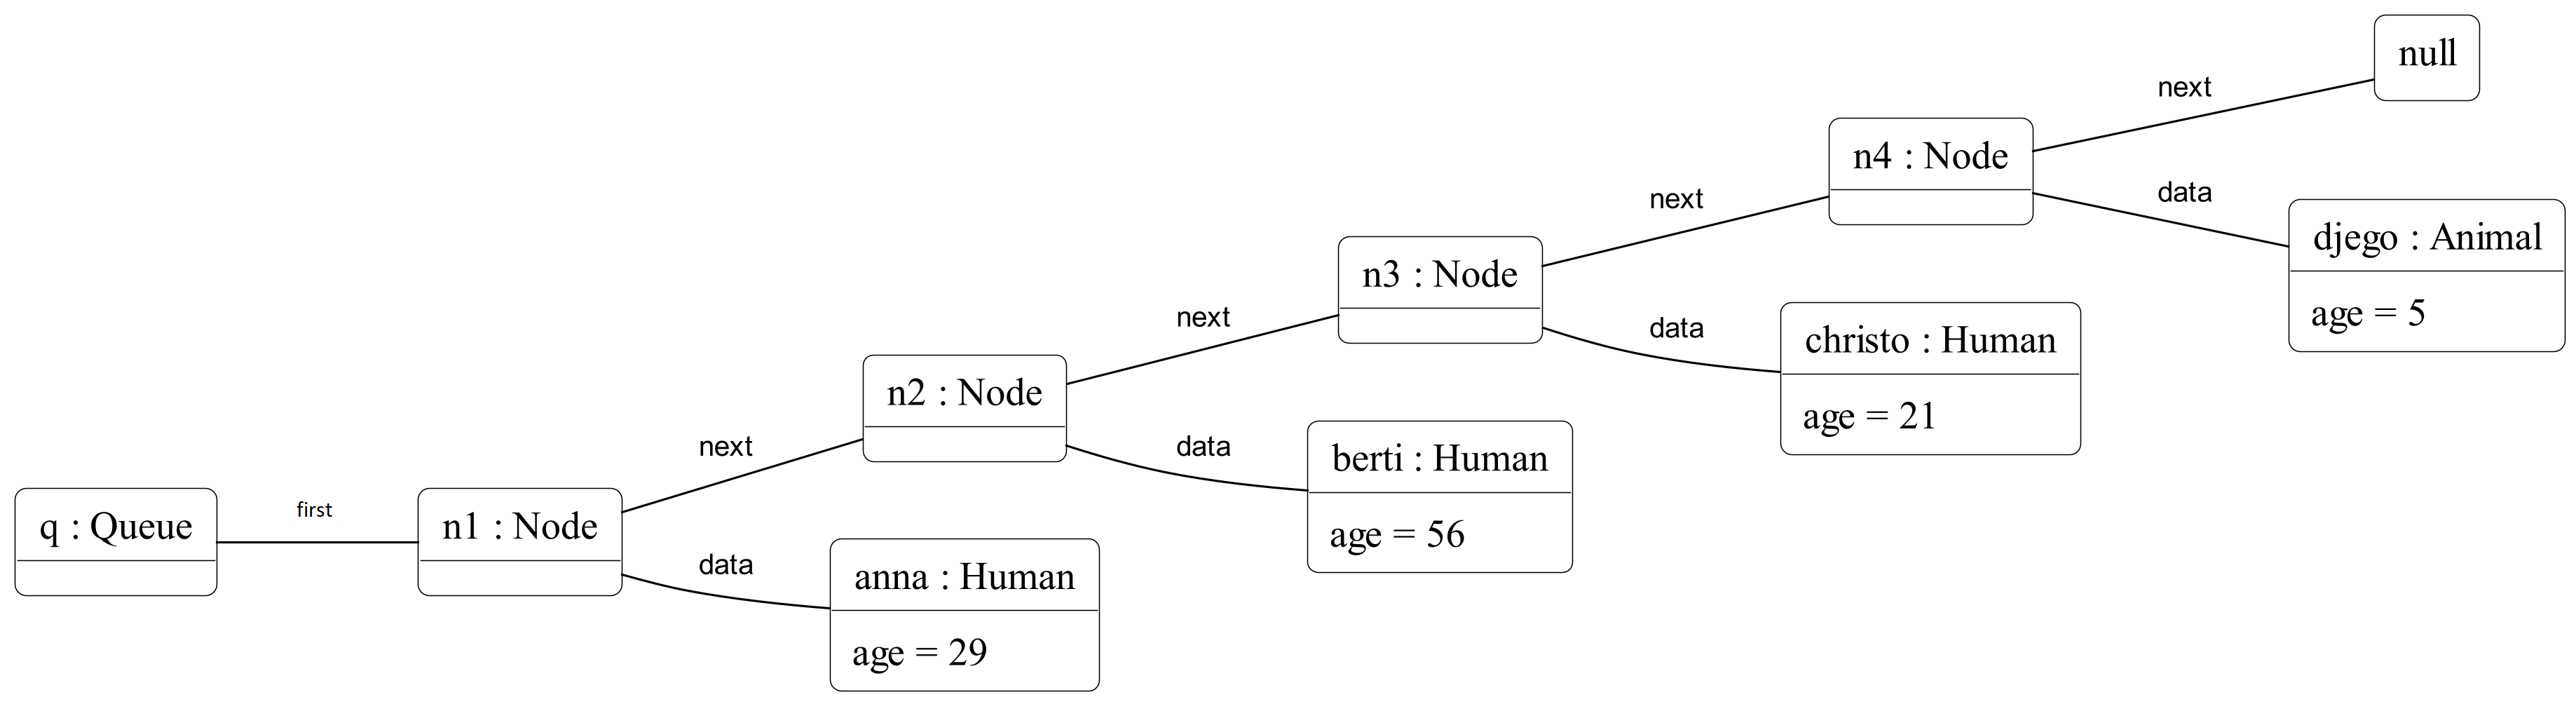
\includegraphics[scale=0.15]{../media/linked_list_nodes_objectdiagram_v2.png}
\end{center}

\subsection{Sequenzdiagramme}

Die Aufgabe des Sequenzdiagramms ist es, Methodenaufrufe - insbesondere über mehrere Objekte hinweg - darzustellen. Jedes Objekt erhält dabei eine sogenannte Lebenslinie. Diese Linie stellt dar, wie lange das Objekt \q{lebt}, da es z.B. auch nur kurzzeitig erzeugt werden könnten. \\
Methodenaufrufe werden durch Pfeile dargestellt und der Methodenname wird über den Pfeil geschrieben. Die Rückgabe wird ebenfalls mit einem Pfeil dargestellt, dieses Mal mit dem Rückgabewert über ihm dargestellt. Der Rückgabepfeil wird häufig gestrichelt dargestellt.\\
Sobald ein Objekt aktiv ist, wird ein Aktivitätsbalken gezeichnet. (I.d.R. gestartet durch einen Methodenaufruf und beendet durch eine Rückgabe). \\
Relevante Attribute können im abgerundeten Kasten am Beginn der Lebenslinie eingetragen werden.
Beispiel aus dem Skript: Längenbestimmung einer verketteten Liste.

\begin{center}
    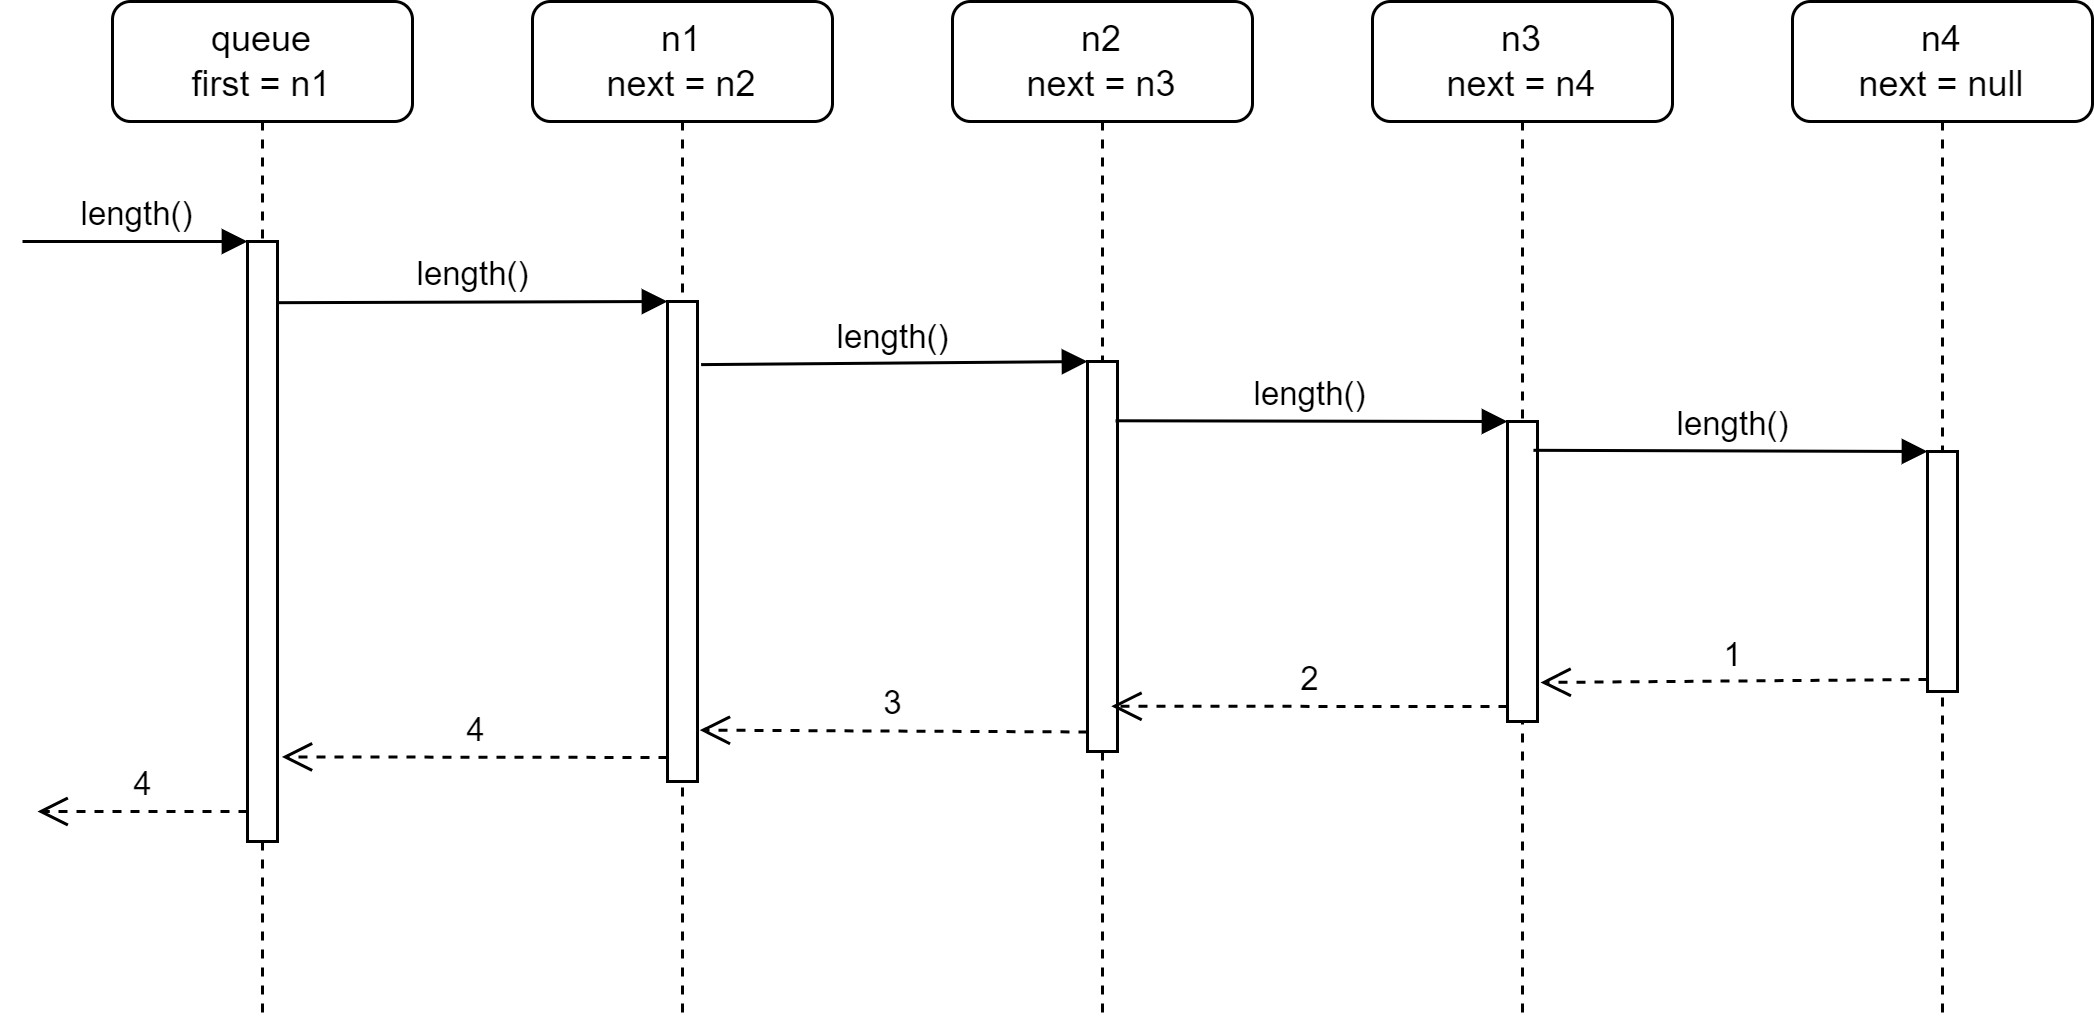
\includegraphics[scale=0.2]{../media/length_sequence.png}
\end{center}

\end{document}